\chapter{Formats de fichiers}
\label{chap-file-formats}
\index{Fichier!formats}\index{Format!de fichier}
Ce chapitre présente les formats des différents fichiers lus ou générés par Unitex. Les
formats des dictionnaires DELAS et DELAF sont déjà présentés aux sections
\ref{section-DELAF-format} et \ref{section-DELAS-format}.

\bigskip
\noindent NOTE: dans ce chapitre, le symbole ¶ représentera le retour à la ligne. Sauf indication
contraire, tous les fichiers texte décrits dans ce chapitre sont codés en Unicode Little-Endian.


\section{Codage Unicode}
\label{unicode-encoding}
\index{Fichier!texte}\index{Unicode}\index{Fichier!\verb+.txt+}\index{Fichier!\verb+.snt+}
Par défaut, les fichiers textes manipulés par Unitex doivent être en Unicode Little-Endian.
Unitex accepte aussi des fichiers Unicode Big-Endian ou UTF-8. Ce codage permet de représenter 65536
caractères en les codant chacun sur 2 octets. En Little-Endian, les octets sont dans l’ordre poids
faible, poids fort. Quand cet ordre est inversé, on parle de codage Big-Endian. Un fichier texte codé
en Little-Endian, Big-Endian or UTF-8 commence par le caractère spécial  (Unicode Byte Order Mark - BOM) de valeur hexadécimale \verb+FF+\,\verb+FE+ (Little-Endian), \verb+FE+\,\verb+FF+ (Big-Endian)
ou \verb+EF+\,\verb+BB+\,\verb+BF+ (UTF-8). 
Parce que UTF-8 n'a pas d'ordre d'octet, l'ajout d'un BOM UTF-8 est optionnel; pour UTF-16 c'est
obligatoire. Les symboles de saut de ligne doivent être codés par les deux caractères
\verb+0D+\,\verb+00+ et \verb+0A+\,\verb+00+ (Little-Endian), 
\verb+00+\,\verb+0D+ et \verb+00+\,\verb+0A+ (Big-Endian), ou \verb+0D+ and \verb+0A+ (UTF-8).

\bigskip
\noindent Considérons le texte suivant:

\bigskip
\texttt{Unitex\P}

\texttt{$\beta$-version\P}

\bigskip
\noindent Voici la représentation en Unicode Little-Endian de ce texte:

\bigskip
\begin{table}[!h]
\begin{center}
\begin{tabular}{|c|c|c|c|c|c|c|c|c|}
\hline
BOM header & U & n & i & t & e & x & \P & $\beta$
\\
\hline
\verb+FF+\,\verb+FE+ & \verb+55+\,\verb+00+ & \verb+6E+\,\verb+00+ & \verb+69+\,\verb+00+ & \verb+74+\,\verb+00+ & \verb+65+\,\verb+00+ & \verb+78+\,\verb+00+
& \verb+0D+\,\verb+00+\,\verb+0A+\,\verb+00+ & \verb+B2+\,\verb+03+
\\
\hline
\hline
- & v & e & r & s & i & o & n & \P
\\
\hline
\verb+2D+\,\verb+00+ & \verb+76+\,\verb+00+ & \verb+65+\,\verb+00+ & \verb+72+\,\verb+00+ & \verb+73+\,\verb+00+ & \verb+69+\,\verb+00+ & \verb+6F+\,\verb+00+
& \verb+6E+\,\verb+00+ & \verb+0D+\,\verb+00+\,\verb+0A+\,\verb+00+
\\
\hline
\end{tabular}
\caption{Représentation hexadécimale d’un texte Unicode Little-Endian}
\end{center}
\end{table}
\pagebreak
\bigskip
\noindent Voici sa représentation en Unicode Big-Endian:

\bigskip
\begin{table}[!h]
\begin{center}
\begin{tabular}{|c|c|c|c|c|c|c|c|c|}
\hline
BOM header & U & n & i & t & e & x & \P & $\beta$
\\
\hline
\verb+FE+\,\verb+FF+ & \verb+00+\,\verb+55+ & \verb+00+\,\verb+6E+ & \verb+00+\,\verb+69+ & \verb+00+\,\verb+74+ & \verb+00+\,\verb+65+ & \verb+00+\,\verb+78+
& \verb+00+\,\verb+0D+\,\verb+00+\,\verb+0A+ & \verb+03+\,\verb+B2+
\\
\hline
\hline
- & v & e & r & s & i & o & n & \P
\\
\hline
\verb+00+\,\verb+2D+ & \verb+00+\,\verb+76+ & \verb+00+\,\verb+65+ & \verb+00+\,\verb+72+ & \verb+00+\,\verb+73+ & \verb+00+\,\verb+69+ & \verb+00+\,\verb+6F+
& \verb+00+\,\verb+6E+ & \verb+00+\,\verb+0D+\,\verb+00+\,\verb+0A+
\\
\hline
\end{tabular}
\caption{Représentation hexadécimale d’un texte Unicode Big-Endian}
\end{center}
\end{table}

\bigskip
\noindent Voici sa représentation Unicode en UTF-8:

\bigskip
\begin{table}[!h]
\begin{center}
\begin{tabular}{|c|c|c|c|c|c|c|c|c|}
\hline
BOM header & U & n & i & t & e & x & \P & $\beta$
\\
\hline
\verb+EF+\,\verb+BB+\,\verb+BF+ & \verb+55+ & \verb+6E+ & \verb+69+ & \verb+74+ & \verb+65+ & \verb+78+
& \verb+0D+\,\verb+0A+ & \verb+CE+\,\verb+B2+
\\
\hline
\hline
- & v & e & r & s & i & o & n & \P
\\
\hline
\verb+2D+ & \verb+76+ & \verb+65+ & \verb+72+ & \verb+73+ & \verb+69+ & \verb+6F+
& \verb+6E+ & \verb+0D+\,\verb+0A+
\\
\hline
\end{tabular}
\caption{Représentation hexadécimale d’un texte Unicode UTF-8}
\end{center}
\end{table}

\bigskip
\noindent En Unicode Little-Endian, les octets de poids fort et de poids faible ont été inversés, ce qui explique que le caractère d’en-tête soit codé par \verb+FF+\,\verb+FE+ au lieu de \verb+FE+\,\verb+FF+, idem pour \verb+00+\,\verb+0D+ et \verb+00+\,\verb+0A+ qui sont devenus respectivement \verb+0D+\,\verb+00+ and \verb+0A+\,\verb+00+.



\section{Fichiers d’alphabet}
Il y a deux sortes de fichiers d’alphabet : un fichier qui définit les caractères d’une langue
et un fichier indiquant des préférences pour le tri. Le premier est désigné sous le terme
\textit{alphabet}, et le second sous celui \textit{alphabet de tri}.


\subsection{Alphabet}
\index{Alphabet}
Le fichier d’alphabet est un fichier texte décrivant tous les caractères d’une langue, ainsi
que les correspondances entre lettres minuscules et majuscules. Ce fichier doit s’appeler
\verb+Alphabet.txt+ \index{Fichier!\verb+Alphabet.txt+} et doit se trouver dans la racine du
répertoire  de la langue concernée. Sa présence est obligatoire pour qu’Unitex puisse fonctionner.


\bigskip
\noindent Exemple : le fichier d’alphabet de l’anglais doit se trouver dans le répertoire 
\verb+.../English/+

\bigskip
\noindent Chaque ligne du fichier alphabet doit avoir l’une des 3 formes suivantes, suivie par un retour à la ligne :


\begin{itemize}
\item 
\includegraphics[height=0.5cm]{resources/img/korean_letters.png} : un dièse suivi de 2
	caractères $X$ and $Y$ indique que tous les caractères compris entre les caractères $X$ et
	$Y$ sont des lettres. Tous ces caractères sont considérés comme étant à la fois minuscules
	et majuscules. Ce mode est utile pour définir les alphabets des langues asiatiques comme le
	coréen, le chinois ou le japonais où il n’y a pas de distinction de casse et où le nombre de
	caractères rendrait très fastidieuse une énumération complète;


\item \verb+Aa+ : 2 caractères  $X$ et $Y$ indiquent que  $X$ et $Y$ sont des lettres et que  $X$                           est l’équivalent en majuscule de la lettre $Y$.

  \item 
\includegraphics[height=0.3cm]{resources/img/thai_letter.png}: un unique caractère $X$
  	  définit $X$ comme une lettre à la fois minuscule et majuscule. Ce mode est utile pour
  	  définir un caractère asiatique de manière ponctuelle.

\end{itemize}

\bigskip
\noindent Pour certaines langues comme le français, il arrive qu’à une lettre minuscule
correspondent plusieurs majuscules. For example, \texttt{é}, qui peut avoir comme majuscule
soit \verb+E+ ou \texttt{\'E}. Pour exprimer cela, il suffit d’utiliser plusieurs lignes.
L’inverse est également vrai : à une majuscule peuvent correspondre plusieurs minuscules. Ainsi,
\verb+E+ peut être la majuscule de \verb+e+, \texttt{é}, \texttt{è}, \texttt{ë} ou \texttt{ê}. Voici l’extrait du fichier alphabet du français qui définit les différentes lettres 

\verb+e+:

\bigskip
\noindent
\texttt{Ee}\P

\noindent
\texttt{Eé}\P

\noindent
\texttt{\'Eé}\P

\noindent
\texttt{Eè}\P

\noindent
\texttt{\`Eè}\P


\noindent
\texttt{Eë}\P

\noindent
\texttt{\"Eë}\P

\noindent
\texttt{Eê}\P

\noindent
\texttt{\^Eê}\P

\subsection{Alphabet de tri}
\index{Alphabet!trié}
L’alphabet de tri est un fichier texte qui définit les priorités des lettres d’une langue lors
du tri à l’aide du programme \verb+SortTxt+.\index{\verb+SortTxt+}\index{Programmes externes!\verb+SortTxt+} Chaque ligne de ce fichier définit un groupe de lettres. Si un groupe de
lettres $A$ est défini avant un groupe de lettres $B$, n’importe quelle lettre de $A$ sera
inférieure à n’importe quelle lettre de $B$.

\bigskip
\noindent Les lettres d’un même groupe ne sont distinguées que si nécessaire. Par exemple, si
l’on a défini le groupe de lettre \verb+eéèëê+ le mot \verb+ébahi+ sera considéré
comme plus petit que \verb+estuaire+, lui-même plus petit que \verb+été+. Comme les lettres
qui suivent \verb+e+ et \verb+é+  permettaient de classer les mots, on n’a pas cherché à comparer
les lettres \verb+e+ et \verb+é+ car elles sont du même groupe.
En revanche, si l’on compare les mots \verb+chantés+ et \verb+chantes+, \verb+chantes+                                                          sera considéré comme plus petit. En effet, il faut comparer les lettres \verb+e+ et  \verb+é+ pour distinguer ces mots. Comme la lettre \verb+e+ apparaît en premier dans le groupe \verb+eéèëê+, elle est considérée comme inférieure à \verb+é+. Le mot \verb+chantes+ sera donc considéré comme plus petit que le mot \verb+chantés+.

\bigskip
\noindent Le fichier d’alphabet de tri permet de définir des équivalences de caractères. On peut
donc ignorer les différences de casse et d’accent. Par exemple, si l’on veut ordonner les lettres
\verb+b+, \verb+c+, et \verb+d+ sans tenir compte de la casse ni de la cédille, on peut écrire les
lignes suivantes :

\bigskip
\noindent
\texttt{Bb}\P

\noindent
\texttt{Cc\c{C}\c{c}}\P

\noindent
\texttt{Dd}\P

\bigskip
\noindent Ce fichier est facultatif. Lorsqu’aucun alphabet de tri n’est spécifié au programme 
\verb+SortTxt+ celui-ci effectue un tri dans l’ordre d’apparition des caractères dans le codage Unicode.


\section{Graphes}
\index{Graphe!format}
Cette section présente les deux formats de graphes : le format graphique \verb+.grf+
et le format compilé \verb+.fst2+.


\subsection{Format .grf}
\index{Fichier!\verb+.grf+}
Un fichier \verb+.grf+ est un fichier texte contenant des informations de présentation en plus
des informations représentant les contenus des boîtes et les transitions du graphe. Un fichier
 \verb+.grf+ commence par les lignes suivantes:

\bigskip
\verb+#Unigraph+\P

\verb+SIZE 1313 950+\P

\verb+FONT Times New Roman:  12+\P

\verb+OFONT Times New Roman:B 12+\P

\verb+BCOLOR 16777215+\P

\verb+FCOLOR 0+\P

\verb+ACOLOR 12632256+\P

\verb+SCOLOR 16711680+\P

\verb+CCOLOR 255+\P

\verb+DBOXES y+\P

\verb+DFRAME y+\P

\verb+DDATE y+\P

\verb+DFILE y+\P

\verb+DDIR y+\P

\verb+DRIG n+\P

\verb+DRST n+\P

\verb+FITS 100+\P

\verb+PORIENT L+\P

\verb+#+\P

\bigskip
\noindent La première ligne \verb+#Unigraph+ est une ligne de commentaire. Les lignes suivantes définissent les valeurs des paramètres de présentation du graphe :


\begin{itemize}
  \item \verb+SIZE x y+ : définit la largeur  \verb+x+ et la hauteur \verb+y+ du graphe en pixels;
  
  \item \verb+FONT name:xyz+ : définit la police utilisée pour afficher le contenu des boîtes.
  	  \verb+name+ représente le nom de la police. \verb+x+ indique si la police doit être en
  	  gras ou non. Si \verb+x+ vaut \verb+B+, cela indique que la police doit être en gras. Pour
  	  une police normale, \verb+x+ doit être un espace. De la même manière, \verb+y+ vaut
  	  \verb+I+ si la police doit être en italique, un espace sinon. \verb+z+ représente la
  	  taille de la police;

  \item \verb+OFONT name:xyz+ : définit la police utilisée pour afficher les transductions. Les
  	  paramètres \verb+name+, \verb+x+, \verb+y+, et \verb+z+ sont définis de la même manière
  	  que pour \verb+FONT+;
  
  \item \verb+BCOLOR x+ : définit la couleur de l’arrière-plan du graphe. \verb+x+ représente la
  	  couleur au format RGB;
  \item \verb+FCOLOR x+ : définit la couleur de dessin du graphe. \verb+x+ représente la couleur au
  	  format RGB;

  \item \verb+ACOLOR x+ : définit la couleur utilisée pour dessiner les lignes des boîtes qui
  	  correspondent à des appels à des sous-graphes. \verb+x+ représente la couleur au format
  	  RGB;

  \item \verb+SCOLOR x+ : définit la couleur utilisée pour écrire le contenu des boîtes de
  	  commentaires (i.e. les boîtes qui ne sont reliées à aucune autre). \verb+x+ représente la
  	  couleur au format RGB;

  \item \verb+CCOLOR x+ : définit la couleur utilisée pour dessiner les boîtes sélectionnées. 
  \verb+x+ représente la couleur au format RGB;

  \item \verb+DBOXES x+ : cette ligne est ignorée par Unitex. Elle est conservée par souci de
  	  compatibilité avec les graphes Intex ;

  \item \verb+DFRAME x+ : dessine ou non un cadre autour du graphe selon que \verb+x+ vaut
  	  \verb+y+, ou \verb+n+;

  \item \verb+DDATE x+ : affiche ou non la date en bas du graphe selon que \verb+x+ vaut
  	  \verb+y+, ou \verb+n+;

  \item \verb+DFILE x+ : affiche ou non le nom du fichier en bas du graphe selon que \verb+x+ vaut
  	  \verb+y+, ou \verb+n+;

  \item \verb+DDIR x+ : affiche ou non le chemin complet d’accès au fichier en bas du graphe selon
  	  que \verb+x+ vaut \verb+y+, ou \verb+n+; Cette option n’est prise en compte que si le
  	  paramètre \verb+DFILE+ a la valeur \verb+y+;

  \item \verb+DRIG x+ : dessine le graphe de droite à gauche ou de gauche à droite selon que
  	  \verb+x+ vaut \verb+y+, ou \verb+n+;

  \item \verb+DRST x+ : cette ligne est ignorée par Unitex. Elle est conservée par souci de
  	  compatibilité avec les graphes Intex ;

  \item \verb+FITS x+ : cette ligne est ignorée par Unitex. Elle est conservée par souci de
  	  compatibilité avec les graphes Intex ;

  \item \verb+PORIENT x+ : cette ligne est ignorée par Unitex. Elle est conservée par souci de
  	  compatibilité avec les graphes Intex ;

  \item \verb+#+ : cette ligne est ignorée par Unitex. Elle sert à indiquer la fin des informations
  	  d’en-tête.

\end{itemize}

\bigskip
\noindent  Les lignes suivantes donnent le contenu et la position des boîtes du graphe. Les lignes
suivantes correspondent à un graphe reconnaissant un chiffre :


\bigskip
\verb+3+\P

\verb+"<E>" 84 248 1 2 +\P

\verb+"" 272 248 0 +\P

\verb$s"1+2+3+4+5+6+7+8+9+0" 172 248 1 1 $\P

\bigskip
\noindent La première ligne indique le nombre de boîtes du graphe, immédiatement suivi d’un
retour à la ligne. Ce nombre ne doit jamais être inférieur à 2, car un graphe est toujours
sensé posséder un état initial et un état final.


\bigskip
\noindent Les lignes suivantes définissent les boîtes du graphe. Les boîtes sont numérotées à partir
de $0$. Par convention, l’état $0$ est l’état initial et l’état $1$ est l’état final. Le contenu de
l’état final doit toujours être vide.


\bigskip
\noindent Chaque boîte du graphe est définie par une ligne qui doit avoir le format suivant :

\bigskip
\textit{contenu X Y N transitions \P}

\bigskip
\noindent \textit{contenu} est une chaîne de caractères entourée de guillemets qui représente le contenu de la boîte. Cette chaîne peut éventuellement être précédée d’un \verb+s+                                                                        dans le cas d’un graphe Intex importé ; ce caractère est alors ignoré par Unitex. Le contenu de la chaîne est le texte qui a été entré dans le contrôle de texte de l’éditeur de graphes. Le tableau
\ref{table10-2} donne le codage des deux séquences spéciales qui ne sont pas codées telles quelles dans les fichiers \verb+.grf+:

\bigskip
\begin{table}[h]
\begin{center}
\begin{tabular}{|c|c|}
\hline
Séquence dans l’éditeur de graphe & Séquence dans le fichier \verb+.grf+
\\
\hline
\verb$"$ & \verb$\"$
\\
\hline
\verb$\"$ & \verb$\\\"$
\\
\hline
\end{tabular}
\caption{Codage des séquences spéciales\label{table10-2}}
\end{center}
\end{table}

\bigskip
\noindent NOTE: les caractères compris entre \verb+<+ et \verb+>+ ou entre \verb+{+ et \verb+}+ ne
sont pas interprétés. Ainsi, le caractère \verb$+$ contenu dans la chaîne \verb$"le <A+Conc>"$ n’est
pas interprété comme un séparateur de lignes, car le motif \verb$<A+Conc>$ est interprété en
priorité.

\bigskip
\noindent \textit{X} and \textit{Y} représentent les coordonnées de la boîte en pixels. La figure
\ref{fig-box-coordinates} montre comment ces coordonnées sont interprétées par Unitex.


\begin{figure}[!h]
\begin{center}
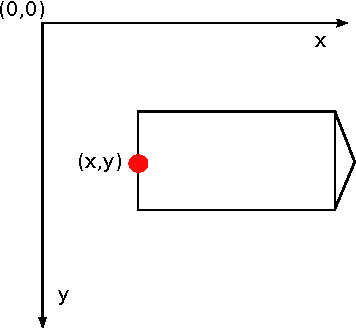
\includegraphics[width=7cm]{resources/img/repere.pdf}
\caption{Interprétation des coordonnées des boîtes\label{fig-box-coordinates}}
\end{center}
\end{figure}

\bigskip
\noindent \textit{N} représente le nombre de transitions qui sortent de la boîte. Ce nombre doit
toujours valoir $0$ pour l’état final.

\bigskip
\noindent Les transitions sont définies par les numéros des boîtes vers lesquelles elles pointent.

\bigskip
\noindent Chaque ligne de définition de boîte doit se terminer par un espace suivi d’un retour à la
ligne.

\subsection{Format .fst2}
\index{Fichier!\verb+.fst2+}
Un fichier \verb+.fst2+ est un fichier texte qui décrit un ensemble de graphes. Voici un exemple
de fichier \verb+.fst2+ file:

\bigskip
\verb+0000000002+\P

\verb+-1 NP+\P

\verb+: 1 1 +\P

\verb+: 2 2 -2 2 +\P

\verb+: 3 3 +\P

\verb+t +\P

\verb+f +\P

\verb+-2 Adj+\P

\verb+: 6 1 5 1 4 1 +\P

\verb+t +\P

\verb+f +\P

\verb+%<E>+\P

\verb+%the/DET+\P

\verb+%<A>/ADJ+\P

\verb+%<N>+\P

\verb+%nice+\P

\verb+@pretty+\P

\verb+%small+\P

\verb+f+\P

\bigskip
\noindent La première ligne représente le nombre de graphes codés dans le fichier. Le début de
chaque graphe est identifié par une ligne indiquant le numéro et le nom du graphe (
	(\verb+-1 NP+ et \verb+-2 Adj+ dans le fichier ci-dessus).

\bigskip
\noindent Les lignes suivantes décrivent les états du graphe. Si l’état est terminal, la ligne débute par le caractère \verb+t+ et par le caractère \verb+:+ sinon. Pour chaque état, la liste des transitions est une suite éventuellement vide de couples d’entiers :


\begin{itemize}
  \item le premier entier indique le numéro d’étiquette ou de sous-graphe correspondant à la
   transition. Les étiquettes sont numérotées à partir de 0. Les sous-graphes sont représentés par des entiers négatifs, ce qui explique que les numéros précédant les noms
   des graphes soient négatifs ;


  \item le deuxième entier représente le numéro de l’état d’arrivée de la transition. Dans
chaque graphe, les états sont numérotés à partir de 0. Par convention, l’état 0 d’un
graphe est son état initial.


\end{itemize}

\bigskip
\noindent Chaque ligne de définition d’état doit se terminer par un espace. La fin de chaque graphe est marquée par une ligne contenant un \verb+f+ suivi d’un espace et d'un retour à la ligne.

\bigskip
\noindent Les étiquettes sont définies après le dernier graphe. Si la ligne débute par le caractère
\verb+@+,cela signifie que le contenu de l’étiquette doit être recherché sans variante de casse.
Cette information n’est utile que lorsque l’étiquette est un mot. Si la ligne débute par le
caractère \verb+%+, les variantes de casse sont autorisées. Si une étiquette porte une transduction,
les séquences d’entrée et de sortie sont séparées par le caractère
 \verb+/+  (exemple : \verb+the/DET+). Par convention, la première étiquette doit toujours être le
 mot vide (\verb+<E>+), et ce, même si cette étiquette n’est utilisée dans aucune transition.


\bigskip
\noindent La fin du fichier est indiquée par une ligne contenant le caractère f suivi d’un retour à la ligne.




\section{Textes}
Cette section présente les différents fichiers utilisés pour représenter des textes.
\subsection{Fichiers .txt}
\index{Fichier!\verb+.txt+}\index{\verb+{S}+}\index{Étiquette lexicale}\index{Séparateur!de phrases}
\label{section-texts}
Les fichiers \verb+.txt+ doivent être des fichiers texte codés en Unicode Little-Endian. Ces
fichiers ne doivent pas contenir d’accolade ouvrante ou fermante, à moins qu’elles soient utilisées
pour écrire un séparateur de phrase (\verb+{S}+) ou une étiquette lexicale valide
(\verb+{aujourd'hui,.ADV}+). Les retours à la ligne doivent être codés par les deux caractères
spéciaux de valeurs hexadécimales \verb+000D+ and \verb+000A+.


\subsection{Fichiers .snt}
\index{Fichier!\verb+.snt+}
\verb+.snt+ sont des fichiers \verb+.txt+ qui ont été prétraités par Unitex. Ces fichiers ne doivent
pas contenir de tabulation. Ils ne doivent pas non plus contenir plusieurs espaces ou retours à la
ligne consécutifs. Les seules accolades autorisées dans des fichiers \verb+.snt+ sont celles du
séparateur de phrases \verb+{S}+\index{\verb+{S}+}\index{Séparateur!de phrases} et celles des
étiquettes lexicales (\verb+{aujourd'hui,.ADV}+)\index{Étiquette lexicale}.


\subsection{Fichier text.cod}
\index{Fichier!\verb+text.cod+}
Le fichier \verb+text.cod+ est un fichier binaire contenant une suite d’entiers représentant le
texte. Chaque entier \verb+i+ renvoie au token d’indice \verb+i+ dans le fichier \verb+tokens.txt+                          Ces entiers sont codés sur 4 octets.


\bigskip
\noindent NOTE : les tokens sont numérotés à partir de 0.

\subsection{Fichier tokens.txt}
\index{Fichier!\verb+tokens.txt+}
Le fichier \verb+tokens.txt+ est un fichier texte contenant la liste de toutes les unités lexicales
du texte. La première ligne de ce fichier indique le nombre d’unités contenues dans le fichier.
Les unités sont séparées par des retours à la ligne. Quand une séquence est trouvée dans le
texte avec des variantes de casse, chaque variante est codée par une unitée distincte.

\bigskip
\noindent NOTE : les retours à la ligne éventuellement présents dans le fichier \verb+.snt+                                                                              sont codés comme des espaces. Il n’y a donc jamais d’unité codant le retour à la ligne.


\subsection{Fichier tok\_by\_alph.txt et tok\_by\_freq.txt}
\index{Fichier!\verb+tok_by_alph.txt+}\index{Fichier!\verb+tok_by_freq.txt+}
Ces deux fichiers sont des fichiers texte qui contiennent la liste des unités lexicales triée
par ordre alphabétique ou par ordre de fréquence.

\bigskip
\noindent Dans le fichier \verb+tok_by_alph.txt+, chaque ligne est composée d’une unité, suivie par
le caractère tabulation et le nombre d’occurrences de cette unité dans le texte.

\bigskip
\noindent Les lignes du fichier \verb+tok_by_freq.txt+ sont formées sur le même principe, mais le
nombre d’occurrences apparaît avant le caractère tabulation et l’unité.


\subsection{Fichier enter.pos}
\index{Fichier!\verb+enter.pos+}
Ce fichier est un fichier binaire contenant la liste des positions des retours à la ligne dans le
fichier \verb+.snt+. Chaque position est l’indice dans le fichier text.cod d’un retour à la ligne
ayant été remplacé par un espace. Ces positions sont des entiers codés sur 4 octets.





\section{Automate du texte}

\subsection{Fichier text.tfst}
\label{section-tfst-format}
\index{Fichier!\verb+text.tfst+}
Le fichier \verb+text.tfst+ représente l’automate du texte. C'est un fichier texte  qui commence par une ligne comportant dix chiffres qui indiquent le nombre de phrases contenues dans l'automate. Ensuite, pour chaque phrase, on dispose de l'en-tête suivante:


\begin{itemize}
\item \verb+$XXX+\P : \verb+XXX+ = numéro de la phrase;

\item \verb+foo foo foo...+\P : texte de la phrase;

\item \verb+a/b c/d e/f g/h...+\P : pour chaque token de la phrase, il y a une 
	paire \verb+x/y+: \verb+x+ est l'index du token dans le fichier
	\verb+tokens.txt+, \verb+y+ est sa longueur en caractères;

\item \verb+X_Y+\P : \verb+X+ est l'offset du premier token de la phrase, en tokens depuis le début
du texte; \verb+Y+ est identique mais l'offset représente le nombre de caractères.
\end{itemize}


\bigskip
\noindent Ensuite, tous les états de l'automate sont codés, un par ligne. Si l'état est final, la
ligne commence par \verb+t+. Sinon, elle commence par \verb+:+. Toutes les transitions sont écrites
sous la forme de paires \verb+x y+, \verb+x+ étant le nombre de tag, \verb+y+ étant le nombre
d'états de destination. Remarquons que contrairement au format \verb+.fst2+, les lignes doivent
finir par un espace. La dernière ligne de la liste d'états contient \verb+f+. 

\bigskip
\noindent Enfin, tous les les tags sont codés. Par convention, le premier tag est toujours épsilon:
\bigskip
\noindent \verb$@<E>$\P

\noindent \verb$.$\P


\bigskip
\noindent D'autres étiquettes doivent être soit des unités lexicales ou des entrées au format DELAF
entre accolades. Elles sont codées comme suit:

\bigskip
\noindent \verb$@STD$\P

\noindent \verb$@$\textit{content}\P

\noindent \verb$@$\textit{a}\verb$.$\textit{b}\verb$.$\textit{c}\verb$-$
\textit{x}\verb$.$\textit{y}\verb$.$\textit{z}\P

\noindent \verb$.$\P


\bigskip
\noindent \textit{contenu} est le contenu du tag. Les informations \textit{a.b.c-x.y.z}
décrivent la zone du texte couverte par le tag:

\begin{itemize}
\item \textit{a}: offset de début en tokens depuis le début de la phrase;
\item \textit{b}: offset de début en caractères depuis le début du premier;
	token du tag;
\item \textit{c}: offset de début en lettres logiques depuis le premier caractère du 
	tag. Ces informations sont utiles pour le coréen, parce qu'un tag
    	    représent une séquence de caractères Jamo qui apparaissent à l'intérieur d'un Hangul. L'offset en caractères n'est donc pas assez précis;\index{Jamo}\index{Hangul}
    \item \textit{x}: offset de fin en tokens depuis le début de la phrase;
    \item \textit{y}: offset de fin en caractères depuis le début du dernier token du tag;
    \item \textit{z}: de fin en lettres logiques depuis le dernier caractère du
    	    the tag. Dans des automates de phrase coréen, des formes de surface vides peuvent correspondre à des mots vides du texte. Dans ces cas, \textit{z} a la valeur $-1$.
\end{itemize}

\bigskip
\noindent La définition de tag se termine par une ligne qui contient \verb+f+.

\bigskip
\noindent Exemple : Voici le fichier correspondant au texte \textit{He is
drinking orange juice.}

\bigskip
\noindent\verb$0000000001$\P

\noindent\verb+$1+\P

\noindent\verb$He is drinking orange juice. $\P

\noindent\verb$0/2 1/1 2/2 1/1 3/8 1/1 4/6 1/1 5/5 6/1 1/1$\P

\noindent\verb$0_0$\P

\noindent\verb$: 2 1 1 1$\P

\noindent\verb$: 4 2 3 2$\P

\noindent\verb$: 7 3 6 3 5 3$\P

\noindent\verb$: 10 5 9 4 8 4$\P

\noindent\verb$: 12 5 11 5$\P

\noindent\verb$: 13 6$\P

\noindent\verb$t$\P

\noindent\verb$f$\P

\noindent\verb$@<E>$\P

\noindent\verb$.$\P

\noindent\verb$@STD$\P

\noindent\verb$@{He,he.N:s:p}$\P

\noindent\verb$@0.0.0-0.1.0$\P

\noindent\verb$.$\P

\noindent\verb$@STD$\P

\noindent\verb$@{He,he.PRO+Nomin:3ms}$\P

\noindent\verb$@0.0.0-0.1.0$\P

\noindent\verb$.$\P

\noindent\verb$@STD$\P

\noindent\verb$@{is,be.V:P3s}$\P

\noindent\verb$@2.0.0-2.1.0$\P

\noindent\verb$.$\P

\noindent\verb$@STD$\P

\noindent\verb$@{is,i.N:p}$\P

\noindent\verb$@2.0.0-2.1.0$\P

\noindent\verb$.$\P

\noindent\verb$@STD$\P

\noindent\verb$@{drinking,drinking.A}$\P

\noindent\verb$@4.0.0-4.7.0$\P

\noindent\verb$.$\P

\noindent\verb$@STD$\P

\noindent\verb$@{drinking,drinking.N:s}$\P

\noindent\verb$@4.0.0-4.7.0$\P

\noindent\verb$.$\P

\noindent\verb$@STD$\P

\noindent\verb$@{drinking,drink.V:G}$\P

\noindent\verb$@4.0.0-4.7.0$\P

\noindent\verb$.$\P

\noindent\verb$@STD$\P

\noindent\verb$@{orange,orange.A}$\P

\noindent\verb$@6.0.0-6.5.0$\P

\noindent\verb$.$\P

\noindent\verb$@STD$\P

\noindent\verb$@{orange,orange.N:s}$\P

\noindent\verb$@6.0.0-6.5.0$\P

\noindent\verb$.$\P

\noindent\verb$@STD$\P

\noindent\verb$@{orange juice,orange juice.N+XN+z1:s}$\P

\noindent\verb$@6.0.0-8.4.0$\P

\noindent\verb$.$\P

\noindent\verb$@STD$\P

\noindent\verb$@{juice,juice.N+Conc:s}$\P

\noindent\verb$@8.0.0-8.4.0$\P

\noindent\verb$.$\P

\noindent\verb$@STD$\P

\noindent\verb$@{juice,juice.V:W:P1s:P2s:P1p:P2p:P3p}$\P

\noindent\verb$@8.0.0-8.4.0$\P

\noindent\verb$.$\P

\noindent\verb$@STD$\P

\noindent\verb$@.$\P

\noindent\verb$@9.0.0-9.0.0$\P

\noindent\verb$.$\P

\noindent\verb$f$\P






\subsection{Fichier text.tind}
\index{Fichier!\verb+text.tind+}
Le fichier \verb+text.tind+ utilisé pour sauter à l'octet d'offset correct dans le fichier
\verb+text.tfst+ quand on veut charger une phrase donnée. C'est un fichier binaire qui contient $4
\times N$ octets,où $N$ est le nombre de phrases. Il donne l'offset de départ de chaque phrase sous
la forme d'une suite de 4 octets en little-endian.


\subsection{Fichier cursentence.grf}
\label{section-cursentence_grf}
\index{Fichier!\verb+cursentence.grf+}
Le fichier  \verb+cursentence.grf+ est généré par Unitex lors de l’affichage d’un automate de
phrase. Le programme \verb+Fst2Grf+ construit un fichier \verb+.grf+ représentant l’automate d’une phrase à partir du fichier \verb+text.fst2+.

\bigskip
\noindent NOTE: les sorties des boîtes sont utilisées pour coder les offsets, tels que définis dans
\verb+.tfst+. Les offsets sont séparés par des espaces. Voici, par exemple, quelques lignes qui representent la première phrase d'\textit{Ivanhoe}:

\bigskip
\noindent \verb$"Ivanhoe/0 0 0 0 6 0" 100 200 2 3 4 $\P
 
\noindent \verb$"{by,by.PART}/2 0 0 2 1 0" 220 150 2 5 6 $\P

\noindent \verb$"{by,by.PREP}/2 0 0 2 1 0" 220 50 2 5 6 $\P

\noindent \verb$"{Sir,sir.N+Hum:s}/4 0 0 4 2 0" 310 200 1 7$\P 




\subsection{Fichier sentenceN.grf}
Lorsque l’utilisateur modifie l’automate d’une phrase, cet automate est sauvegardé sous
le nom \verb+sentenceN.grf+, où \verb+N+ représente le numéro de la phrase.

un tel graphe contient des offsets dans les sorties des boîtes du graphe (voir note 
section \ref{section-cursentence_grf}).


\subsection{Fichier cursentence.txt}
\index{Fichier!\verb+cursentence.txt+}
Lors de l'extraction de l'automate phrase, le texte de la phrase est
enregistré dans le fichier appelé \verb+cursentence.txt+. Ce fichier est utilisé par Unitex pour
afficher le texte de la phrase sous l'automate. Ce fichier contient le texte de la phrase, suivie
d'un saut de ligne.

\subsection{The cursentence.tok file}
\index{Fichier!\verb+cursentence.tok+}
Lors de l'extraction de l'automate phrase, les numéros de tokens qui composent la phrase sont
enregistrés dans un fichier nommé \verb+cursentence.tok+. Ce fichier contient une ligne par token,
chaque ligne étant composée de 2 entiers \verb$x y$: \verb$x$ est le numéro de token, \verb$y$ est
sa longueur en caractères.

\bigskip
\noindent Voici le contenu de ce fichier pour la première phrase d'\textit{Ivanhoe}:

\bigskip
\noindent \verb$0 7$\P \verb$         $\textit{Ivanhoe}

\noindent \verb$1 1$\P \verb$         $\texttt{\char `\ }

\noindent \verb$2 2$\P \verb$         $\textit{by}

\noindent \verb$1 1$\P \verb$         $\texttt{\char `\ }

\noindent \verb$3 3$\P \verb$         $\textit{Sir}

\noindent \verb$1 1$\P \verb$         $\texttt{\char `\ }

\noindent \verb$4 6$\P \verb$         $\textit{Walter}

\noindent \verb$1 1$\P \verb$         $\texttt{\char `\ }

\noindent \verb$5 5$\P \verb$         $\textit{Scott}

\noindent \verb$1 1$\P \verb$         $\texttt{\char `\ }


\subsection{Fichiers tfst\_tags\_by\_freq.txt et tfst\_tags\_by\_alph.txt}
\index{Fichier!\verb+tfst_tags_by_freq.txt+}
\index{Fichier!\verb+tfst_tags_by_alph.txt+}
Ces fichiers contiennent tous les tags qui apparaissent dans l'automate du texte classés par fréquence et par ordre alphabétique.


\section{Concordances}
\subsection{Fichier concord.ind}
\index{Fichier!\verb+concord.ind+}
Le fichier \verb+concord.ind+ est l’index des occurrences trouvées par les programmes \verb+Locate+
ou \verb+LocateTfst+ lors de l’application d’une grammaire. C’est un fichier texte qui contient les
positions de début et de fin de chaque occurrence, éventuellement accompagnées d’une chaîne de
caractères si la concordance a été obtenue en prenant en compte les éventuelles transductions de la
grammaire. Voici un exemple de fichier :


\bigskip
\verb$#M$\P

\verb$59.0.0 63.3.0 the[ADJ= greater] part$\P

\verb$67.0.0 71.4.0 the beautiful hills$\P

\verb$87.0.0 91.3.0 the pleasant town$\P

\verb$123.0.0 127.4.0 the noble seats$\P

\verb$157.0.0 161.5.0 the fabulous Dragon$\P

\verb$189.0.0 193.3.0 the Civil Wars$\P

\verb$455.0.0 459.11.0 the feeble interference$\P

\verb$463.0.0 467.6.0 the English Council$\P

\verb$566.0.0 570.10.0 the national convulsions$\P

\verb$590.0.0 594.5.0 the inferior gentry$\P

\verb$626.0.0 630.11.0 the English constitution$\P

\verb$696.0.0 700.4.0 the petty kings$\P

\verb$813.0.0 817.5.0 the certain hazard$\P

\verb$896.0.0 900.5.0 the great Barons$\P

\verb$938.0.0 942.3.0 the very edge$\P

\bigskip
\noindent La première ligne indique dans quel mode de transduction la concordance a été calculée.
Les trois valeurs possibles sont :

\begin{itemize}
  \item \verb+#I+ : les transductions ont été ignorées;

  \item \verb+#M+ : les transductions ont été insérées dans les séquences reconnues (mode MERGE);
  \index{MERGE}
  
  \item \verb+#R+ : les transductions ont remplacé les séquences reconnues (mode REPLACE).
  \index{REPLACE}
\end{itemize}

\bigskip
\noindent Chaque occurrence est décrite par une ligne. Les lignes commencent par les positions de
début et de fin de l’occurrence. Ces positions correspondent aux offsets
définis dans le fichier tag \verb$.tfst$  (voir \ref{section-tfst-format}).

\bigskip
\noindent Si le fichier comporte la ligne d’en-tête \verb+#I+, la position de fin de chaque
occurrence est immédiatement suivie d’un retour à la ligne. Dans le cas contraire, elle est suivie
d’un espace et d’une chaîne de caractères. En mode REPLACE, cette chaîne correspond à la
transduction produite pour la séquence reconnue. En mode MERGE, elle représente la séquence reconnue
dans laquelle ont été insérées les transductions. En mode MERGE ou REPLACE, c’est cette chaîne qui
est affichée dans la concordance. Si les transductions ont été ignorées, le contenu de l’occurrence
est extrait du fichier texte.



\subsection{Fichier concord.txt}
\index{Fichier!\verb+concord.txt+}
Le fichier \verb+concord.txt+ est un fichier texte représentant une concordance. Chaque occurrence
est codée par une ligne composée de 3 chaînes de caractères séparées par le caractère de tabulation
et qui représentent le contexte gauche, l’occurrence (éventuellement
modifiée par des transductions) et le contexte droit.



\subsection{Fichier concord.html}
\index{Fichier!\verb+concord.html+}
Le fichier \verb+concord.html+ est un fichier \verb+HTML+ qui représente une concordance. Ce fichier
est codé en UTF-8.\index{UTF-8}

\bigskip
\noindent Le titre de la page est le nombre d’occurrences qu’elle décrit. Les lignes de la
concordance sont codées par des lignes où les occurrences sont considérées comme des liens
hypertextes. La référence associée à chacun de ces liens est de la forme~:

\medskip
\verb+<a href="X Y Z">+

\medskip
\noindent \verb+X+ et \verb+Y+ représentent les positions de début et de fin de l’occurrence en caractères
dans le fichier \verb+name_of_text.snt+. \verb+Z+ représente le numéro de la phrase dans laquelle
apparaît cette occurrence.

\bigskip
\noindent Tous les espaces sont codés comme des espaces insécables (\verb+&nbsp;+ in HTML), ce qui
permet de conserver l’alignement des occurrences, même si l’une d’elles, se trouvant en début de
fichier, a un contexte gauche complété avec des espaces.


\bigskip
\noindent NOTE : dans le cas d’une concordance construite avec le paramètre glossanet, le fichier
HTML obtenu a la même structure, sauf en ce qui concerne les liens. Dans ces concordances, les
occurrences sont des liens réels renvoyant vers le serveur web de l’application GlossaNet. Pour plus
d’information sur GlossaNet, consulter les liens sur le site web
d’Unitex.(http://www-igm.univ-mlv.fr/~unitex).\index{GlossaNet}

\bigskip
\noindent Voici un exemple de fichier:

\bigskip

\verb$<html lang=en>$\P

\verb$<head>$\P

\verb$$\P

\verb$   <meta http-equiv="Content-Type" content="text/html;$

\verb$         charset=UTF-8">$\P

\verb$   <title>6 matches</title>$\P

\verb$</head>$\P

\verb$<body>$\P

\verb$<table border="0" cellpadding="0" width="100%" $

\verb$       style="font-family: 'Arial Unicode MS'; font-size: 12">$\P

\verb$<font face="Courier new" size=3>$\P

\verb$on, there <a href="116 124 2">extended</a>&nbsp;i&nbsp;<br>$\P

\verb$&nbsp;extended <a href="125 127 2">in</a>&nbsp;ancient&nbsp;<br>$\P

\verb$&nbsp;Scott {S}<a href="32 34 2">IN</a>&nbsp;THAT PL&nbsp;<br>$\P

\verb$STRICT of <a href="61 66 2">merry</a>&nbsp;Engl&nbsp;<br>$\P

\verb+S}IN THAT <a href="40 48 2">PLEASANT</a>&nbsp;D&nbsp;<br>+\P

\verb+&nbsp;which is <a href="84 91 2">watered</a>&nbsp;by&nbsp;<br>+\P

\verb$</font>$\P

\verb$</td></table></body>$\P

\verb$</html>$\P


\bigskip
\noindent La figure \ref{fig-example-concordance-2} montre la page correspondant au fichier
ci-dessus.

\begin{figure}[!h]
\begin{center}
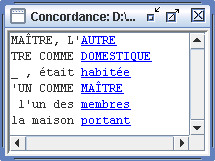
\includegraphics[width=5cm]{resources/img/fig10-2.png}
\caption{Exemple de concordance \label{fig-example-concordance-2}}
\end{center}
\end{figure}



\subsection{Fichier diff.html}
\index{Fichier!\verb+diff.html+}
Le fichier \verb+diff.html+ est une page \verb+HTML+ qui montre les différences entre deux concordances. Ce fichier est encodé en UTF-8.\index{UTF-8} Voici un exemple de fichier (des retours à la ligne ont été introduits pour la mise en page) :



\begin{verbatim}
<html>
<head>
<meta http-equiv="Content-Type" content="text/html;
charset=UTF-8">
<style type="text/css">
a.blue {color:blue; text-decoration:underline;}
a.red {color:red; text-decoration:underline;}
a.green {color:green; text-decoration:underline;}
</style>
</head>
<body>
<h4>
<font color="blue">Blue:</font> identical sequences<br>
<font color="red">Red:</font> similar but different sequences<br>
<font color="green">Green:</font> sequences that occur in only
one of the two concordances<br>
<table border="1" cellpadding="0" style="font-family: Courier new;
font-size: 12">
<tr><td width="450"><font color="blue">ed in ancient times
<u>a large forest</u>, covering the greater par</font></td>
<td width="450"><font color="blue">ed in ancient times
<u>a largeforest</u>, covering the greater par</font></td>
</tr>
<tr><td width="450"><font color="green">ge forest, covering
<u>the greater part</u>&nbsp;of the beautiful hills </font>
</td>
<td width="450"><font color="green"></font></td>
</tr>
</table>
</body>
</html>
\end{verbatim}


\section{Dictionnaires du texte}
Le programme \verb+Dico+ produit plusieurs fichiers qui représentent les dictionnaires.

\subsection{dlf et dlc}
\index{Fichier!\verb+dlf+}
\index{Fichier!\verb+dlc+}

\verb+dlf+ et \verb+dlc+ sont des dictionnaires de mots simples et composés au format DELAF
format (voir section \ref{section-DELAF-format}).

\subsection{err}
\index{Fichier!\verb+err+}
Ce fichier contient les mots inconnus, un par ligne.

\subsection{tags\_err}
\index{Fichier!\verb+tags_err+}
Ce fichier contient les mots inconnus, un par ligne. La différence avec le fichier \verb+err+ est que dans celui-ci les mots simples reconnus dans le fichier \verb+tags.ind+ n'apparaissent pas.

\subsection{tags.ind}
\index{Fichier!\verb+tags.ind+}
\label{section-tags-ind}
Ce fichier a le même format que \verb+concord.ind+ il s'obtient en mode MERGE ou REPLACE mais son en-tête est \verb+#T+. Remarquons que les sorties ne commence pas par un slash.
 


\section{Dictionnaires}
La compression des dictionnaires DELAF par le programme \verb+Compress+ produit 2 fichiers : un
fichier \verb+.bin+  qui représente l’automate minimal des formes fléchies du dictionnaire, et un
fichier \verb+.inf+ qui contient les formes comprimées permettant de reconstruire les lignes du
dictionnaire à partir des formes fléchies. Cette section décrit le format de ces deux types de
fichiers, ainsi que le format du fichier \verb+CHECK_DIC.TXT+, qui contient le résultat de
la vérification d’un dictionnaire.

\index{\verb+Compress+}\index{Programmes externes!\verb+Compress+}

\index{DELAF}\index{Dictionnaire!DELAF}

\subsection{Fichier .bin}
\index{Fichier!\verb+.bin+}
Un fichier \verb$.bin$ est un fichier binaire représentant un automate. Les 4 premiers octets du
fichier représentent un entier indiquant la taille du fichier en octets. Les états de l’automate
sont ensuite codés de la manière suivante :

\begin{itemize}

  \item les 2 premiers octets indiquent si l’état est terminal ainsi que le nombre de transitions
qui en sortent. Le bit le plus fort vaut 0 si l’état est terminal et 1 sinon. Les 15 autres
bits codent le nombre de transitions.

  \bigskip Exemple : un état non terminal avec 17 transitions est codé par la séquence hexadécimale
  8011

  \bigskip \item si l’état est terminal, les 3 octets suivants codent l’indice dans le fichier
  \verb+.inf+ de la forme comprimée à utiliser pour reconstruire les lignes de dictionnaires pour
  cette forme fléchie.

  \bigskip Exemple : si l’état renvoie à la forme comprimée d’indice 25133, la séquence hexadécimale
  correspondante est \verb+00622D+
  

  \bigskip \item chaque transition sortante est ensuite codée sur 5 octets. Les 2 premiers octets
  codent le caractère étiquetant la transition, et les 3 suivants codent la position en octets dans
  le fichier \verb+.bin+ de l’état d’arrivée. Les transitions d’un état sont codées les unes à la
  suite des autres.


  \bigskip Exemple : une transition étiquetée par le caractère A pointant vers l’état dont la description débute au $50106$ème , octet sera représenté par la séquence hexadécimale \verb+004100C3BA+.

\end{itemize}

\bigskip
\noindent Par convention, le premier état de l’automate est l’état initial.

\subsection{Fichier.inf}
\index{Fichier!\verb+.inf+}
Un fichier \verb+.inf+ est un fichier texte décrivant les formes comprimées associées à un fichier \verb+.bin+. Voici un exemple de fichier \verb+.inf+ file:

\bigskip
\verb$0000000006$\P

\verb$_10\0\0\7.N$\P

\verb$.PREP$\P

\verb$_3.PREP$\P

\verb$.PREP,_3.PREP$\P

\verb$1-1.N+Hum:mp$\P

\verb$3er 1.N+AN+Hum:fs$\P

\bigskip
\noindent La première ligne du fichier indique le nombre de formes comprimées qu’il contient.
Chaque ligne peut contenir une ou plusieurs formes comprimées. S’il y a plusieurs formes,
celles-ci doivent être séparées par des virgules. Chaque forme comprimée est formée d’une
séquence permettant de retrouver une forme canonique à partir d’une forme fléchie, suivie
par la séquence de codes grammaticaux, sémantiques et flexionnels associés à l’entrée.


\bigskip
\noindent Le mode de compression de la forme canonique varie en fonction de la forme fléchie.
Si les deux formes sont exactement identiques, la forme comprimée se résume aux informations
grammaticales, sémantiques et flexionnelles, comme c’est le cas dans la ligne suivante :

\bigskip
\verb$.N+Hum:ms$

\bigskip
\noindent Si les formes sont différentes, le programme de compression découpe les deux formes en
unités. Ces unités peuvent être soit un espace, soit un tiret, soit une séquence de caractères
ne contenant ni espace ni tiret. Ce mode de découpage permet de prendre efficacement en
compte les flexions des mots composés.


\bigskip
\noindent Si les formes fléchies et canonique ne comportent pas le même nombre d’unités, le
programme code la forme canonique par le nombre de caractères à retrancher de la forme fléchie,
suivi des caractères à ajouter. Ainsi, la première ligne du fichier ci-dessus correspond à la ligne
de dictionnaire :


\bigskip
\verb+James Bond,007.N+

\bigskip
\noindent Comme la séquence \verb+James Bond+ contient trois unités et \verb+007+ seulement une, la
forme canonique est codée par \verb+_10\0\0\7+. Le caractère \verb+_+ indique que les deux formes
n’ont pas le même nombre d’unités. Le nombre qui suit (ici 10) indique le nombre de caractères à
retrancher. La séquence \verb+\0\0\7+ qui suit ce nombre indique que l’on doit ensuite ajouter la
séquence \verb+007+. Les chiffres sont précédés du caractère \verb+\+ pour ne pas être confondus
avec le nombre de caractères à retrancher.


\bigskip
\noindent Lorsque les deux formes ont le même nombre d’unités, les unités sont comprimées deux
à deux. Si les deux unités sont composées d’un espace ou d’un tiret, la forme comprimée de
l’unité est l’unité elle-même, comme c’est le cas dans la ligne suivante :


\bigskip
\verb$0-1.N:p$

\bigskip
\noindent qui est la sortie pour \verb$battle-axes,battle-axe.N:p$

\bigskip
\noindent Cela permet de conserver une certaine visibilité dans le fichier \verb+.inf+ lorsque le dictionnaire contient des mots composés.


\bigskip
\noindent Lorsque au moins une des unités n’est ni un espace ni un tiret, la forme comprimée est
composée du nombre de caractères à retrancher suivi de la séquence de caractères à ajouter.
Ainsi, la ligne de dictionnaire :

\bigskip
\noindent
\texttt{premi\`ere partie,premier parti.N+AN+Hum:fs}

\bigskip
\noindent est codée par la ligne :

\bigskip
\verb$3er 1.N+AN+Hum:fs$

\bigskip
\noindent Le code \verb+3er+ indique que l’on doit retrancher 3 caractères à la séquence
\texttt{premi\`ere} et lui ajouter les caractères \verb+er+  pour obtenir \verb+premier+. Le 
\verb+1+ indique que l’on doit simplement retirer un caractère à \verb+partie+ pour obtenir la
séquence  \verb+parti+. Le nombre \verb+0+ est utilisé lorsqu’on veut indiquer que l’on ne doit
supprimer aucun caractère.


\subsection{Fichier information sur un dictionnaire}
\index{Fichier!information dictionnaire}
Dans le cadre "Apply lexical resources", il est possible d'obtenir quelques informations sur
un dictionnaire par click droit. Ces informations sont associées aux dictionnaires \verb+biniou.bin+
ou \verb+biniou.fst2+ à l'aide d'un texte brut nommé \verb+biniou.txt+, situé dans le même
répertoire.

\subsection{Fichier CHECK\_DIC.TXT}
\index{Fichier!\verb+CHECK_DIC.TXT+}\index{\verb+CheckDic+}\index{Programmes
externes!\verb+CheckDic+}
Ce fichier est produit par le programme de vérification de dictionnaire \verb+CheckDic+.                                                                                             Il s’agit d’un fichier texte qui donne des informations sur le dictionnaire analysé, et se décom-
pose en quatre parties.


\bigskip
\noindent La première partie donne la liste, éventuellement vide, de toutes les erreurs de syntaxe
trouvées dans le dictionnaire : absence de la forme fléchie ou de la forme canonique, absence
de code grammatical, ligne vide, etc. Chaque erreur est décrite par le numéro de la ligne
concernée, un message décrivant la nature de l’erreur, ainsi que le contenu de la ligne. Voici
un exemple de message :


\begin{verbatim}
Line 12451: unexpected end of line
garden,N:s
\end{verbatim}

\bigskip
\noindent Les deuxième et troisième parties donnent respectivement les listes de codes grammaticaux
et/ou sémantiques et flexionnels. Afin de prévenir des erreurs de codage, le programme signale les
codes qui contiennent des espaces, des tabulations ou des caractères non ASCII. Ainsi, si un
dictionnaire grec contient le code \verb+ADV+ où le caractère \verb+A+ est le \verb+A+ grec au lieu du \verb+A+ latin, le programme signalera l’avertissement suivant :

\begin{verbatim}
ADV warning: 1 suspect char (1 non ASCII char): (0391 D V)
\end{verbatim}

\bigskip
\noindent Les caractères non ASCII sont indiqués par leur numéro de caractère en hexadécimal.Dans
l’exemple ci-dessus, le code \verb+0391+ représente le \verb+A+ grec. Les espaces sont indiqués par
la séquence \verb+SPACE+:

\begin{verbatim}
Km s warning: 1 suspect char (1 space): (K m SPACE s)
\end{verbatim}

\bigskip
\noindent Lorsqu’on vérifie le dictionnaire suivant :

\begin{verbatim}
1,2 et 3!,.INTJ 
abracadabra,INTJ 
supercalifragilisticexpialidocious,.INTJ
damned,. INTJ
Paul,.N+Hum+Hum
eat,.V:W:P1s:Ps:P1p:P2p:P3p
\end{verbatim}

\bigskip
\noindent on obtient le fichier \verb+CHECK_DIC.TXT+ suivant :

\bigskip
\verb$Line 1: unprotected comma in lemma$\P

\verb$1,2 et 3!,.INTJ $\P

\verb$Line 2: unexpected end of line$\P

\verb$abracadabra,INTJ $\P

\verb$Line 5: duplicate semantic code$\P

\verb$Paul,.N+Hum+Hum$\P

\verb$Line 6: an inflectional code is a subset of another$\P

\verb$eat,.V:W:P1s:Ps:P1p:P2p:P3p$\P

\verb$-----------------------------------$\P

\verb$-------------  Stats  -------------$\P

\verb$-----------------------------------$\P

\verb$File: D:\My Unitex\English\Dela\axe.dic$\P

\verb$Type: DELAF$\P

\verb$6 lines read$\P

\verb$2 simple entries for 2 distinct lemmas$\P

\verb$0 compound entry for 0 distinct lemma$\P

\verb$-----------------------------------$\P

\verb$----  All chars used in forms  ----$\P

\verb$-----------------------------------$\P

\verb$a (0061)$\P

\verb$c (0063)$\P

\verb$d (0064)$\P

\verb$e (0065)$\P

\verb$f (0066)$\P

\verb$g (0067)$\P

\verb$i (0069)$\P

\verb$l (006C)$\P

\verb$m (006D)$\P

\verb$n (006E)$\P

\verb$o (006F)$\P

\verb$p (0070)$\P

\verb$r (0072)$\P

\verb$s (0073)$\P

\verb$t (0074)$\P

\verb$u (0075)$\P

\verb$x (0078)$\P

\verb$-------------------------------------------------------------$\P

\verb$----    2 grammatical/semantic codes used in dictionary  ----$\P

\verb$-------------------------------------------------------------$\P

\verb$INTJ$\P

\verb$ INTJ warning: 1 suspect char (1 space): (SPACE I N T J)$\P

\verb$-----------------------------------------------------$\P

\verb$----    0 inflectional code used in dictionary  -----$\P

\verb$-----------------------------------------------------$\P

\bigskip
\noindent Remarquons que les codes flexionnels de \verb+eat+ ne sont pas signalés, puisque
une erreur s'est produite dans cette ligne.


\section{Fichiers ELAG}
\subsection{Fichier tagset.de}
\index{Fichier!\verb+tagset.def+}
See section \ref{section-elag-tagset}, page \pageref{section-elag-tagset}.

\subsection{Fichiers .lst}
\index{Fichier!\verb+.lst+}

LES FICHIERS .LST NE SONT PAS CODÉS EN UNICODE.

\bigskip
\noindent Un fichier \verb$.lst$ contient une liste de noms de fichiers \verb$.grf$. Si
le nom d'un fichier n'est pas absolu, il est relatif à l'emplacement du fichier
\verb$elag.lst$. Voici le fichier \verb$elag.lst$ fourni pour le français :


\bigskip
\verb$PPVs/PpvIL.grf$\P

\verb$PPVs/PpvLE.grf$\P

\verb$PPVs/PpvLUI.grf$\P

\verb$PPVs/PpvPR.grf$\P

\verb$PPVs/PpvSeq.grf$\P

\verb$PPVs/SE.grf$\P

\verb$PPVs/postpos.grf$\P

\subsection{.elg files}
\index{Fichier!\verb+.elg+}

Les fichiers \verb$.elg$ contiennent des règles ELAG compilées. Ces fichiers sont au format \verb$.fst2$.


\subsection{Fichier .rul}
\index{Fichier!\verb+.rul+}

LES FICHIERS .RUL NE SONT PAS CODÉS EN UNICODE.

\bigskip
\noindent Un fichier \verb$.rul$ contient différents fichiers \verb$.elg$ qui compose un ensemble de règles
ELAG. Un fichier \verb$.rul$ est constitué d’autant de parties qu’il y a de fichiers  \verb$.elg$. Chaque
partie est composée de la liste des grammaires ELAG qui correspondent à un fichier \verb$.elg$ . Les noms
de fichiers \verb$.elg$ sont entres angles. Les lignes commençant par une tabulation ont valeur de commentaire
et sont ignorées par le programme \verb+Elag+.\index{\verb+Elag+}\index{Programmes externes!\verb+Elag+}
Voici le fichier \verb$elag.rul$ fourni par défaut pour le français :

\bigskip
\verb$    PPVs/PpvIL.elg$\P

\verb$    PPVs/PpvLE.elg$\P

\verb$    PPVs/PpvLUI.elg$\P

\verb$<elag.rul-0.elg>$\P

\verb$    PPVs/PpvPR.elg$\P

\verb$    PPVs/PpvSeq.elg$\P

\verb$    PPVs/SE.elg$\P

\verb$    PPVs/postpos.elg$\P

\verb$<elag.rul-1.elg>$\P

\section{Fichier taggeur}
Cette section présente les fichiers produits et utilisés par les programmes TrainingTagger et
Tagger.

\subsection{Fichier corpus.txt}
\index{Fichier!\verb+corpus.txt+}
\label{section-corpus-file}
Ce fichier est utilisé par le programme TrainingTagger afin de calculer les statistiques pour le
programme Tagger. Il contient des phrases où chaque mot est représenté sur une ligne séparée.

Chaque ligne représentant un mot est constituée d'un mot, simple ou composé, suivie d'une barre
oblique et de l'étiquette du mot.

Cette étiquette est composée d'un code grammatical, parfois suivi d'une\verb$'+'$ et de codes
syntaxiques ou sémantiques. Les codes flexionnels sont spécifiés après un \verb+':'+. Si le mot est
un composé, les mots simples qui y figurent doivent être séparés par un \verb+'_'+. 
Voici un exemple d'un fichier corpus.txt:

\bigskip
\verb$The/DET+Ddef:s$\P

\verb+GATT/N:s+\P

\verb+had/V:I3s+\P

\verb+formerly/ADV+\P

\verb$a/DET+Dind:s$\P

\verb+political/A+\P

\verb+assessment/N:s+\P

\verb+of/PREP+\P

\verb$the/DET+Ddef:s$\P

\verb+behavior/N:s+\P

\verb+of/PREP+\P

\verb+foreign_countries/N:p+\P

\verb+./PONCT+\P

\P

\verb$She/PRO+Nomin:3fs$\P

\verb+closed/V:I3s+\P

\verb+easily/ADV+\P

\verb$her/DET+Poss3fs:p$\P

\verb+eyes/N:p+\P

\verb+when/CONJ+\P

\verb$some/DET+Dadj:p$\P

\verb+infractions/N:p+\P

\verb+might/V:I3p+\P

\verb+appear/V:W+\P

\verb+justified/V:K+\P

\verb+against/PREP+\P

\verb+higher/A+\P

\verb+interests/N:p+\P

\verb+./PONCT+\P

\P

\bigskip
\noindent REMARQUE: Les phrases doivent être délimitées par des lignes vides.

\bigskip
Le format \verb+.txt+ peut également être utilisé (voir section \ref{section-texts}). Chaque mot du
texte doit être représenté par une étiquette lexicale valide
(\verb+{aujourd'hui,.ADV}+)\index{Étiquette lexicale} et les phrases sont délimitées par
\verb+{S}+\index{\verb+{S}+}\index{Délimiteur de phrase}.
Voici l'exemple précédent dans le format \verb+.txt+ :

\bigskip
\verb${The,.DET+Ddef:s}$ \verb${GATT,.N:s}$ \verb${had,.V:I3s}$ \verb${formerly,.ADV}$\\ 
\verb${a,.DET+Dind:s}$ \verb${political,.A}$ \verb${assessment,.N:s}$ \verb${of,.PREP}$\\ 
\verb${the,.DET+Ddef:s}$ \verb${behavior,.N:s}$ \verb${of,.PREP}$ \verb${foreign countries,.N:p}$\\ 
\verb${.,.PONCT}$ \verb${S}$ \verb${She,.PRO+Nomin:3fs}$ \verb${closed,.V:I3s}$ \verb${easily,.ADV}$\\
\verb${her,.DET+Poss3fs:p}$ \verb${eyes,.N:p}$ \verb${when,.CONJ}$ \verb${some,.DET+Dadj:p}$\\
\verb${infraction,.N:p}$ \verb${might,.V:I3p}$ \verb${appear,.V:W}$ \verb${justified,.V:K}$\\
\verb${against,.PREP}$ \verb${higher,.A}$ \verb${interests,.N:p}$ \verb${.,.PONCT}$ \verb${S}$

\subsection{Le fichier de données du taggueur}
\index{Fichier!\verb+train_dict+}
\label{section-training-dict}
The TrainingTagger programme  genère deux fichiers de données (par défaut) utilisé par le programme
Tagger afin de calculer un modèle de Markov caché d'ordre 2. Ces fichiers contiennent des tuples
unigram, bigramme et trigramme extraits du corpus étiqueté corpus.txt. Les tuples sont composés soit
d'une séquence de 2 ou 3 tags (pour calculer la probabilité de transition) ou d'un mot précédé par 0
ou 1 tag (pour calculer la probabilité émise). Les unités dans un tuple doivent être séparées par
une tabulation. Ces tuples sont suivis par la séquence de délimiteurs ",." et ensuite un nombre
entier représentant le nombre d'occurrences de ce tuple dans le corpus.

\bigskip

\noindent Les noms de fichiers sont suffixés par "cat" ou "morph". Dans la premier, les tuples sont
composés tags de codes grammaticaux, syntaxiques et sémantiques. Dans le second, les tuples sont
composés de tags de codes grammaticaux, syntaxiques et sémantiques parfois suivis par un
\verb+':'+ et des codes flexionnels.
Voici un exemple d'un fichier de données avec des tags de type "cat" :

\bigskip
\verb+the,.9630+\P

\verb+those,.236+\P

\verb+eyes,.32+\P

\verb$DET+Ddef	 the,.9630$\P

\verb$DET+Ddem	 those,.140$\P

\verb$PRO+Pdem	 those,.96$\P

\verb+N		   eyes,.32+\P

\verb+DET	 N,.62541+\P

\verb+PREP	DET  N,.25837+\P

\P

\bigskip

\noindent Voici un exemple d'un fichier de données avec des tags de type "morph" :

\bigskip
\verb+the,.9630+\P

\verb+those,.236+\P

\verb+eyes,.32+\P

\verb$DET+Ddef:s	 the,.4437$\P

\verb$DET+Ddef:p	 the,.5193$\P

\verb$DET+Ddem:p	 those,.140$\P

\verb$PRO+Pdem:p	 those,.96$\P

\verb+N:p		   eyes,.32+\P

\verb+DET:s	 N:s,.18489+\P

\verb+PREP	  DET:s  N:s,.6977+\P

\P

\bigskip
\noindent Une ligne spécifique est ajoutée à des fichiers de données afin de déterminer si le fichier contient des tags de type "cat" ou "morph".

Cette ligne contient \verb+CODE FEATURES+ suivie soit le nombre 0 pour "cat" tags ou 1 pour
"morph".

\bigskip
\noindent REMARQUE: À l'étape finale, TrainingTagger comprime ces deux fichiers de données au format \verb+.bin+.


\section{Fichier de configuration}
\subsection{Fichier Config}
\index{Fichier!\verb+Config+}
Lorsque l’utilisateur modifie ses préférences pour une langue donnée, celles-ci sont sauvegardées
dans un fichier texte nommé \verb+Config+ qui se trouve dans le répertoire de la langue courante. Ce
fichier a la syntaxe suivante (l’ordre des lignes peut varier) :



\bigskip
\verb$#Unitex configuration file of 'paumier' for 'English'$\P

\verb$#Fri Oct 10 15:18:06 CEST 2008$\P

\verb$TEXT\ FONT\ NAME=Courier New$\P

\verb$TEXT\ FONT\ STYLE=0$\P

\verb$TEXT\ FONT\ SIZE=10$\P

\verb$CONCORDANCE\ FONT\ NAME=Courier new$\P

\verb$CONCORDANCE\ FONT\ HTML\ SIZE=12$\P

\verb$INPUT\ FONT\ NAME=Times New Roman$\P

\verb$INPUT\ FONT\ STYLE=0$\P

\verb$INPUT\ FONT\ SIZE=10$\P

\verb$OUTPUT\ FONT\ NAME=Arial Unicode MS$\P

\verb$OUTPUT\ FONT\ STYLE=1$\P

\verb$OUTPUT\ FONT\ SIZE=12$\P

\verb$DATE=true$\P

\verb$FILE\ NAME=true$\P

\verb$PATH\ NAME=false$\P

\verb$FRAME=true$\P

\verb$RIGHT\ TO\ LEFT=false$\P

\verb$BACKGROUND\ COLOR=-1$\P

\verb$FOREGROUND\ COLOR=-16777216$\P

\verb$AUXILIARY\ NODES\ COLOR=-3289651$\P

\verb$COMMENT\ NODES\ COLOR=-65536$\P

\verb$SELECTED\ NODES\ COLOR=-16776961$\P

\verb$PACKAGE\ NODES\ COLOR=-2302976$\P

\verb$CONTEXT\ NODES\ COLOR=-16711936$\P

\verb$CHAR\ BY\ CHAR=false$\P

\verb$ANTIALIASING=false$\P

\verb$HTML\ VIEWER=$\P

\verb$MAX\ TEXT\ FILE\ SIZE=2097152$\P

\verb$ICON\ BAR\ POSITION=West$\P

\verb$PACKAGE\ PATH=D\:\\repository$\P

\verb$MORPHOLOGICAL\ DICTIONARY=D\:\\MyUnitex\\English\\Dela\\zz.bin$\P

\verb$MORPHOLOGICAL\ NODES\ COLOR=-3911728$\P

\verb$MORPHOLOGICAL\ USE\ OF\ SPACE=false$\P


\bigskip
\noindent Les deux premières lignes sont des lignes de commentaires. Les trois lignes suivantes
indiquent le nom, le style et la taille de la police utilisée pour afficher les textes, les
dictionnaires, les unités lexicales, les phrases de l’automate du texte, etc.


\bigskip
\noindent The \verb$CONCORDANCE FONT NAME$ et \verb$CONCORDANCE FONT HTML SIZE$ définissent le nom et la taille de la police à utiliser pour afficher les concordances en HTML. La taille de la police doit être comprise entre 1 et 7.



\bigskip
\noindent Les paramètres \verb$INPUT FONT ...$ et \verb$OUTPUT FONT ...$ définissent le nom, le
style et la taille des polices utilisées pour afficher les chemins et les transductions des graphes.



\bigskip
\noindent Les 10 paramètres suivants correspondent aux paramètres précisés dans les en-têtes des
graphes. Le tableau \ref{tab-parameters} décrit ces correspondances.

\begin{table}[h]
\begin{center}
\begin{tabular}{|c|c|}
\hline
Paramètres dans le fichier \verb+Config+ file & Paramètres dans un fichier \verb+.grf+ file
\\
\hline
\verb$DATE$ & \verb$DDATE$
\\
\hline
\verb$FILE NAME$ & \verb$DFILE$
\\
\hline
\verb$PATH NAME$ & \verb$DDIR$
\\
\hline
\verb$FRAME$ & \verb$DFRAME$
\\
\hline
\verb$RIGHT TO LEFT$ & \verb$DRIG$
\\
\hline
\verb$BACKGROUND COLOR$ & \verb$BCOLOR$
\\
\hline
\verb$FOREGROUND COLOR$ & \verb$FCOLOR$
\\
\hline
\verb$AUXILIARY NODES COLOR$ & \verb$ACOLOR$
\\
\hline
\verb$COMMENT NODES COLOR$ & \verb$SCOLOR$
\\
\hline
\verb$SELECTED NODES COLOR$ & \verb$CCOLOR$
\\
\hline
\end{tabular}
\caption{Signification des paramètres\label{tab-parameters}}
\end{center}
\end{table}

\bigskip
\noindent Le paramètre \verb+PACKAGE NODES+ définit la couleur des appels à des sous-graphes du
répertoire de dépôt.

\bigskip
\noindent Le paramètre \verb+CONTEXT NODES+ définit la couleur des boîtes correspondant à des débuts
ou fins de contextes.

\bigskip
\noindent Le paramètre \verb+CONTEXT NODES+ indique si la langue courante doit être traitée en mode
caractère par caractère ou non.

\bigskip
\noindent Le paramètre \verb+ANTIALIASING+ indique si les graphes ainsi que les automates de phrases
doivent être affichés par défaut avec l’effet d’antialiasing.

\bigskip
\noindent Le paramètre \verb+HTML VIEWER+ indique le nom du navigateur à utiliser pour afficher les
concordances. Si aucun nom de navigateur n’est précisé, les concordances sont affichées
dans une fenêtre d’Unitex.

\bigskip
\noindent Le paramètre \verb+MAX TEXT FILE SIZE+ n'est plus utlisé.

\bigskip
\noindent Le paramètre \verb+ICON BAR POSITION+ définit la position de la barre d’icônes dans les fenêtres de graphes.


\bigskip
\noindent Le paramètre \verb+PACKAGE PATH+ définit le répertoire de dépôt à utiliser pour cette langue.

\bigskip
\noindent Le paramètre \verb+MORPHOLOGICAL DICTIONARY+ indique la liste des dictionnaires du mode morphologique, séparés par des points virgules.

\bigskip
\noindent Le paramètre \verb+MORPHOLOGICAL NODES COLOR+ définit la couleur des étiquettes du mode morphologique \verb+$<+ et \verb+$>+.

\bigskip
\noindent Le paramètre \verb+MORPHOLOGICAL USE OF SPACE+ indique si le programme
\verb+Locate+ peut commencer en reconnaissant les espaces. (par défaut c'est non)


\subsection{Fichier system\_dic.def}
\index{Fichier!\verb+system_dic.def+}
Le fichier \verb+system_dic.def+ est un fichier texte décrivant la liste des dictionnaires du
système à appliquer par défaut. Ce fichier se trouve dans le répertoire de la langue courante.
Chaque ligne correspond à un nom de fichier \verb+.bin+ file.                                                         Les dictionnaires du système doivent se trouver dans le répertoire du système, à l’intérieur du
sous-répertoire \verb+(langue courante)/Dela+.\index{Fichier!\verb+.bin+}
Voici un exemple de fichier :


\bigskip
\verb$delacf.bin$\P

\verb$delaf.bin$\P

\subsection{Fichier user\_dic.def}
\index{Fichier!\verb+user_dic.def+}
Le fichier \verb+user_dic.def+ est un fichier texte décrivant la liste des dictionnaires de
l’utilisateur à appliquer par défaut. Ce fichier se trouve dans le répertoire de la langue courante
et a le même format que le fichier \verb+system_dic.def+. 
Les dictionnaires de l’utilisateur doivent se trouver dans le sous-répertoire \verb+(langue courante)/Dela+ du répertoire personnel de l’utilisateur.


\subsection{Fichiers (nom d’utilisateur).cfg et .unitex.cfg}
\index{Fichier!\verb+.cfg+}
Sous Linux et Mac OS, Unitex considère que le répertoire personnel de l’utilisateur se nomme \verb+unitex+ et
qu’il se trouve dans son répertoire racine (\verb+$HOME+). Si vous voulez changer cet emplacement
par défaut, un fichier \verb+.unitex.cfg+ est créé dans votre répertoire personnel, et il contient
le chemin vers votre répertoire Unitex privé. Ce fichier est un fichier UTF8. Si \verb+.unitex.cfg+
ne contient pas un chemin Linux valide vers un répertoire existant, il est ignoré\,\footnote{Cela
permet de lancer Unitex tantôt sous Linux, tantôt sous Windows, sur des fichiers partagés~: le chemin Windows vers le
répertoire Unitex personnel est indiqué dans \texttt{.unitex.cfg}, et Unitex l’ignore quand on le lance
sous Linux.}.


\bigskip
Sous Windows, il n’est pas toujours possible d’associer un répertoire par défaut à un
utilisateur. Pour remédier à cela, Unitex crée pour chaque utilisateur un fichier \verb+.cfg+
contenant le chemin de son répertoire Unitex personnel. Ce fichier est sauvegardé sous le nom
\verb+(nom d’utilisateur).cfg+ dans le sous-répertoire \verb+Users+ du répertoire Unitex système. Si l’utilisateur
n’a pas les droits pour écrire dans ce répertoire, un fichier \verb+.unitex.cfg+ est sauvegardé
dans le répertoire du profil utilisateur~:
\begin{itemize}
\item dans \verb+Documents and Settings\(user login)+ sous Windows XP
\item dans \verb+Users\(user login)+ sous WindowsVista ou une version plus récente.
\end{itemize}

\bigskip
\noindent ATTENTION : CE FICHIER N’EST PAS EN UNICODE ET LE CHEMIN DU RÉPERTOIRE PERSONNEL N’EST PAS
SUIVI PAR UN RETOUR À LA LIGNE.


\section{Fichiers CasSys}

\subsection{Fichiers de  configuration CasSys csc}

Pour mémoriser la liste des transducteurs d'une cascade CasSys, nous utilisons un fichier texte
(csc) dans lequel chaque ligne contient le chemin vers un transducteur suivi du mode de sortie
(fusionner / remplacer) à appliquer à ce transducteur.
Le format d'une ligne du fichier csc est : Name\_and\_path\_of\_transducer  Merge
Voici un exemple de fichier de cascade csc:

\ttfamily
"C:$\backslash$apps$\backslash$my\_unitex$\backslash$French$\backslash$Graphs$\backslash$grf1.fst2" Merge

"C:$\backslash$apps$\backslash$my\_unitex$\backslash$French$\backslash$Graphs$\backslash$grf2.fst2" Replace
\rmfamily

\section{Plusieurs autres fichiers}
Pour chaque texte, Unitex crée plusieurs fichiers contenant des informations destinées à être
affichées dans l’interface graphique. Cette section décrit ces différents fichiers.



\subsection{Fichier dlf.n, dlc.n, err.n et tags\_err.n}
\index{Fichier!\verb+dlf.n+}\index{Fichier!\verb+dlc.n+}\index{Fichier!\verb+err.n+}\index{Fichier!\verb+tags_err.n+}
\index{Fichier!\verb+dlf+}\index{Fichier!\verb+dlc+}\index{Fichier!\verb+err+}\index{Fichier!\verb+tags_err+}
Ces trois fichiers sont des fichiers texte se trouvant dans le répertoire du texte. Ils contiennent
respectivement les nombres de lignes des fichiers \verb+dlf+, \verb+dlc+, \verb+err+ et
\verb+tags_err+. Ces nombres sont suivis par un retour à la ligne.



\subsection{Fichier stat\_dic.n}
\index{Fichier!\verb+stat_dic.n+}
Ce fichier est un fichier texte se trouvant dans le répertoire du texte. Il est formé de trois
lignes, contenant les nombres de lignes des fichiers \verb+dlf+, \verb+dlc+ and \verb+err+.

\subsection{Fichier stats.n}
\index{Fichier!\verb+stats.n+}
Ce fichier texte se trouve dans le répertoire du texte et contient une ligne de la forme
suivante :


\bigskip
\verb$3949 sentence delimiters, 169394 (9428 diff) tokens, 73788 (9399)$

\verb$simple forms, 438 (10) digits$\P

\bigskip
\noindent Les nombres indiqués s’interprètent de la façon suivante :

\begin{itemize}
  \item \verb+sentence delimiters+: nombre de séparateurs de phrases
  (\verb+{S}+);\index{\verb+{S}+}
  \index{Séparateur!de phrases}

  \item \verb+tokens+: nombre total d’unités lexicales du texte. Le nombre précédant \verb+diff+
  indique le nombre d’unités différentes;

  \item \verb+simple forms+: nombre total dans le texte d’unités lexicales composées de lettres. Le
  	  nombre entre parenthèses représente le nombre d’unités lexicales différentes qui sont
  	  composées de
lettres ;

  \item \verb+digits+: nombre total dans le texte de chiffres. Le nombre entre parenthèses indique
le nombre de chiffres différents utilisés (au plus 10).

\end{itemize}


\subsection{Fichier concord.n}
\index{Fichier!\verb+concord.n+}
Le fichier \verb+concord.n+ est un fichier texte qui se trouve dans le répertoire du texte. Il
contient des informations sur la dernière recherche de motifs effectuée sur ce texte et se
présente de la manière suivante :


\bigskip
\verb$6 matches$\P

\verb$6 recognized units$\P

\verb$(0.004% of the text is covered)$\P

\bigskip
\noindent La première ligne donne le nombre d’occurrences trouvées, la seconde le nombre d’unités
couvertes par ces occurrences. La troisième ligne indique le rapport entre le nombre d’unités
couvertes et le nombre total d’unités du texte.


\subsection{Fichier concord\_tfst.n}
\index{Fichier!\verb+concord_tfst.n+}
Le fichier \verb+concord_tfst.n+ est un fichier texte qui se trouve dans le répertoire du texte. Il
contient des informations sur la dernière recherche sur l'automate du texte et ressemble à ce qui
suit:

\bigskip
\verb$23 matches(45 outputs)$\P



\subsection{Fichier règles de normalisation}
\index{Fichier!règles de normalisation}
\label{section-normalization-file}
Ce fichier est utilisé par les programmes \verb+Normalization+ et \verb+XMLizer+. Il représente
règles de normalisation. Chaque ligne représente une règle, selon le format suivant ($\longmapsto$
	représente le caractère de tabulation):

\bigskip
\noindent \verb+input sequence+ $\longmapsto$ \verb+output sequence+

\bigskip
\noindent Si vous souhaitez utiliser la tabulation ou le newline, vous devez les déspécialiser
avec un antislash comme ceci:

\bigskip
\noindent
\verb+123\+

\noindent
$\longmapsto$ \verb+ONE_TWO_THREE_NEW_LINE+



\subsection{Fichier de mots interdits}
\index{Fichier!de mots interdits} \label{section-forbidden-words}
Le programme \verb+PolyLex+ requiert un de mots interdits pour le hollandais et le norvégien. Ce fichier texte brut est censé s'appeler \verb+ForbiddenWords.txt+
\index{Fichier!\verb+ForbiddenWords.txt+}. Il doit se trouver dans le répertoire \verb+Dela+
correspondant à la langue courante. Chaque ligne est censée contenir un mot interdit.




\subsection{Fichier de log}
\index{Fichier!de log programmes Unitex} \label{section-log-file}
Le programme \verb+UnitexToolLogger+, si le fichier \verb+unitex_logging_parameters.txt+ 
est trouvé avec un chemin (pour enregistrer les fichiers log) crée un fichier .ulp de log de l'outil 
Unitex en cours d'exécution choisi.

\bigskip

Il crée un fichier \verb+unitex_logging_parameters_count.txt+ qui contient seulement le numéro du
dernier fichier log créé.

Un fichier log (avec l'extension .ulp) est un fichiers zip non comprimés, compatibles avec unzip
et tous les outils unzip standards. On peut le recréer avec zip
d'Infozip (avec les options -0 -X). Il contient ces fichiers:
\begin{itemize}
\item \verb+test_info/command_line.txt+: une liste de paramètres de la ligne de commande utilisée
	pour exécuter l'outil. Il y a un paramètre sur chaque ligne. La première ligne contient la
	valeur de retour, la deuxième ligne le nombre de paramètres;

  \item \verb+test_info/command_line_synth.txt+: une simple ligne avec un résumé de la
ligne de commande utilisée pour exécuter l'outil;

\item \verb+test_info/list_file_in.txt+: une liste des fichiers lus par l'outil.
	La première colonne est la taille du fichier, la seconde est crc32, la troisième le nom du
	fichier;

\item \verb+test_info/list_file_out.txt+: une liste des fichiers créés par l'outil.
  La première colonne est la taille du fichier, la seconde est crc32, la troisième le nom du
  fichier;

  \item \verb+test_info/std_out.txt+: le contenu de sortie standard de la console;

  \item \verb+test_info/std_err.txt+: le contenu de sortie erreurs de la console;

  \item \verb+src/xxx+: une copie du fichier lu par l'outil (nécessaire pour faire fonctionner à
  		  nouveau le log);

  \item \verb+dest/xxx+: une copie du fichier créé par l'outil
\end{itemize}

Si la seconde ligne de unitex\_logging\_parameters.txt contient 0, ces fichiers ne sont pas
enregistrés; si cette ligne contient 1, ils sont enregistrés;

\subsection{Règles typographiques de l'arabe: arabic\_typo\_rules.txt}
\label{subsection-arabic-typo-rules}
\index{Fichier!des règles typographiques de l'arabe}
\index{Fichier!\verb+arabic_typo_rules.txt+}
Pour l'arabe, la recherche dans le dictionnaire peut être paramétrée avec un fichier qui décrit si
certaines variations typographiques sont autorisées ou non. Ce fichier est constitué de lignes comme
celles-ci:

\bigskip
\noindent \verb+fatha omission=YES+

\bigskip
\noindent où \verb+fatha omission+ est le nom de la règle. Pour une description complète de toutes
les règles disponibles, il faut consulter le fichier \verb+Arabic.h+ dans les sources du programme.

\subsection{fichier d'offsets de différence}
\label{subsection-offsets-diff}

Les fichiers d'offsets de différence sont écrit par l'outils Unxmlize, lu par Tokenize, lu et écrit par
DumpOffsets(\ref{section-DumpOffsets}), Normalize(\ref{section-Normalize}), Fst2Txt(\ref{section-Fst2Txt}), Tokenize(\ref{section-Tokenize}), Concord(\ref{section-Concord}) et GrfTest.
\bigskip
Ces fichiers textes sont constituées de lignes contenant 4 entiers A B C D. Chaque ligne correspond à une modification du texte, exprimée de la façon suivante:
\bigskip
l'intervalle [A;B[ du texte *** avant tout traitement *** est remplacé par l'intervalle [C;D[ après traitement, A, B, C et D étant des positions en caractères dans les fichiers textes.
\bigskip

Par exemple, si on applique le programme Normalize sur le texte "Hello  world" (avec deux espaces entre les deux mots), on aura une ligne comme ceci:

\bigskip
\noindent \verb+5 7 5 6+
\bigskip

signifiant qu'une séquence de deux caractères (les 2 espaces) a été remplacée par une séquence d'un seul caractère.

\bigskip

Le principe est donc de produire un nouveau fichier d'offsets pour chaque application de programme modifiant le texte, en prenant en entrée le fichier d'offsets produit par le programme précédent. Ainsi, en regardant le dernier fichier d'offsets produit, on sait que pour chaque ligne A B C D, l'intervalle [C;D[ dans le fichier .snt correspond à l'intervalle [A;B[ dans le fichier .txt de départ


\subsection{fichier d'offsets de zone commune}
\label{subsection-offsets-common}

Les fichiers d'offsets de zone commune sont lu et écrit par DumpOffsets.
\bigskip
Ces fichiers textes sont constituées de lignes contenant 4 entiers A B C D. Chaque ligne correspond à une modification du texte, exprimée de la façon suivante:
\bigskip
l'intervalle [A;B[ du texte original correspond à l'intervalle [C;D[ après traitement, A, B, C et D étant des positions en caractères dans les fichiers textes. Sur chaque ligne, B-A=D-C.
\bigskip

Par exemple, si on applique le programme Normalize sur le texte "Hello world" (avec deux espaces entre les deux mots), on aura une ligne comme ceci:

\bigskip
\noindent \verb+0 5 0 5+
\newline
\noindent \verb+7 12 6 11+
\bigskip

signifiant que les caractère de 0 (inclus) à 5 (non inclus) des deux fichiers contiennent exactement le même texte, et que ceux de 7 (inclus) à 12 (non inclus) du premier texte
contiennent exactement le même texte que ceux de 6 (inclus) à 11 (non inclus) du second.



\subsection{fichier d'offsets uima}
\label{subsection-offsets-uima}
Les fichiers d'offsets uima sont écrit par Tokenize et lu par Concord.

\bigskip
Ces fichiers textes sont constituées de lignes contenant 3 entiers A B C et de texte entre < et >.

\bigskip
Chaque ligne correspond à un token, exprimée de la façon suivante:
Le token numéro A correspond au texte de la position B (inclue) à la position C (non inclus) du fichier d'origine, et le texte de ce token est mentionné entre < et >.
Le numéro de token A correspond au numéro de ligne de tokens.txt où figure ce token (après avoir ajouté 1 pour la ligne d'en-tête de tokens.txt(\ref{Fichier tokens.txt}))

\bigskip
